\section{Authentication and Identity}

%------------------------------------------------
\begin{frame}
\begin{large}
\begin{columns}
\begin{column}{0.5\linewidth}
\begin{block}{Identity}
Who you are.
\end{block}
\end{column}
\begin{column}{0.5\linewidth}
\includeimage[width=\linewidth,height=0.25\textheight]{identity}
\end{column}
\end{columns}
\pause
\begin{columns}
\begin{column}{0.5\linewidth}
\begin{block}{Authentication}
Are you who you claim to be?
\end{block}
\end{column}
\begin{column}{0.5\linewidth}
\includeimage[width=\linewidth,height=0.25\textheight]{authentication}
\end{column}
\end{columns}
\pause
\begin{columns}
\begin{column}{0.5\linewidth}
\begin{block}{Authorization}
What are you allowed to do?
\end{block}
\end{column}
\begin{column}{0.5\linewidth}
\includeimage[width=\linewidth,height=0.25\textheight]{authorization}
\end{column}
\end{columns}
\end{large}
\note{
\begin{block}{Identity}
The identity of somebody is who they claim.
\newline The definition also applies to non-humans (systems).
\end{block}
\begin{block}{Authentication}
Authentication is the act of asserting the identity of someone.
\end{block}
\begin{block}{Authorization}
Authorization is determining whether the user has the permission to do some
action.
\end{block}
}
\end{frame}

%------------------------------------------------
\begin{frametransition}{Identification and confidentiality}
\note{
Authentication is needed when you want to transmit
information and be sure that your correspondent isn't
impersonated by somebody else.
\begin{block}{Confidentiality}
Authentication by itself doesn't imply confidentiality.
For that, we have encryption.
\end{block}
}
\end{frametransition}

%%%%%%%%%%%%%%%%%%%%%%%%%%%%%%%%%%%%%%%%%%%%%%%%%%%%%%%%%%%%%%%%%%%%%%%%%%%%%%
\subsection{Technical introduction}

\subsubsection{HTTP}

\defverbatim[colored]\Lst{
\begin{lstlisting}[style=beamer]
@GET@ @/wiki/Hypertext_Transfer_Protocol@ HTTP/1.1
Host: en.wikipedia.org
User-Agent: Mozilla/5.0 (X11; Linux x86_64; rv:19.0) Gecko/20100101 Firefox/19.0
Accept: text/html,application/xhtml+xml, application/xml;q=0.9,*/*;q=0.8
@Cookie@: @mediaWiki.user.id=m5MFt3bI4Lrx@;
Connection: keep-alive
...
\end{lstlisting}
}

\begin{frame}
\frametitle{How does HTTP work?}
\Lst
\note{
A \emph{request} example.
\begin{itemize}
\item Method: \texttt{GET}, \texttt{POST}, etc.
\item URL: resource path
\item Options: \texttt{Host}, \texttt{Cookie}, etc.
\end{itemize}
The \emph{response} has the same structure.
\begin{block}{Anonymity}
No identifier for a web user.
\par\textbf{Cookies}\\
Data stored on the client's computer.
\par\textbf{Session number}\\
The server identifies its users using a session ID (unique number) for each
client. But... the client can send anything.
\end{block}
}
\end{frame}

\subsubsection*{Cryptography introduction}

\begin{frame}
\frametitle{Symmetric cryptography}
\includeimage[width=0.9\linewidth]{cryptography-symm}
\note{
\begin{block}{Encryption}
Transformation of a message in a way that it is readable only by the
authorized parties.
\end{block}
\begin{block}{Symmetric}
A single key used to encode and decode the messages.
\[ msg \xrightarrow{key} cipher \xrightarrow{key} msg \]
\end{block}
\begin{exampleblock}{Symmetric cryptography algorithms}
AES, DES,...
\end{exampleblock}
}
\end{frame}

\begin{frame}
\frametitle{Asymmetric cryptography}
\includeimage[width=0.8\linewidth]{cryptography-asym}
\note{
\begin{block}{Asymmetric}
A private-public key pair, one is used to encrypt the message, the other to
read it.
\[ msg \xrightarrow{key_{pub}} cipher \xrightarrow{key_{priv}} msg \]
\end{block}
\begin{exampleblock}{Asymmetric cryptography algorithms}
RSA, DSA, ...
\end{exampleblock}
}
\end{frame}

\begin{frame}
\frametitle{Public-private keys}
\includeimage[width=\linewidth,height=\textheight]{ppk}
\note{
By definition, the public key is shared.
\begin{itemize}
\item Encrypt with the recipient's public key
\item Sign with your private key
\end{itemize}
}
\end{frame}

\begin{frame}
\begin{Large}
\begin{tabularx}{\linewidth}{X<{\raggedleft}cX}
\bfseries Symmetric
& 
\includegraphics[width=5mm]{img/vs} &
\bfseries Asymmetric
\\[0.5em]
Fast
& 
\includegraphics[width=5mm]{img/vs} &
Slow
\\[0.2em]
Pre-shared secret
& 
\includegraphics[width=5mm]{img/vs} &
No pre-shared secret
\\[0.2em]
Owner(s) of the secret
& \raisebox{-0.5em}{
\includegraphics[width=5mm]{img/vs}} &
Owner of the private secret
\\[0.2em]
\end{tabularx}
\end{Large}
\note{
\begin{itemize}
\item \textbf{Symmetric}: faster, needs a pre-shared key
	\newline All people holding the key can decrypt the message.
\item \textbf{Asymmetric}: no need for a pre-shared key
	\newline Message can be decrypted by the person holding the right key.
\end{itemize}
\begin{block}{Usual usage}
A connection starts using an \emph{asymmetric} algorithm to exchange keys and
then switches to a \emph{symmetric} algorithm as it is faster.
\end{block}
}
\end{frame}

\begin{frame}
\begin{columns}
\begin{column}{0.8\linewidth}
\flushright\includeimage[width=\linewidth]{hash-joke}
\end{column}
\pause
\begin{column}{0.2\linewidth}
\flushleft\includeimage[width=\linewidth]{salt}
\end{column}
\end{columns}
\note{
Joke: "hachage et salage"
}
\end{frame}

\begin{frame}
\frametitle{Hash + Salt}
\begin{center}
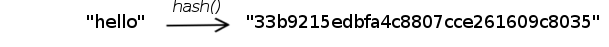
\includegraphics[width=\linewidth]{img/hash1}
\pause
\vspace{1em}
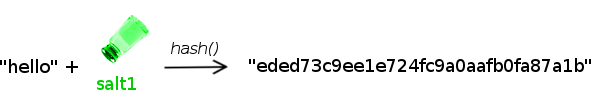
\includegraphics[width=\linewidth]{img/hash2}
\pause
\vspace{1em}
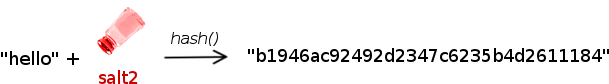
\includegraphics[width=\linewidth]{img/hash3}
\end{center}
\note{
Ensure passwords are hashed with a standard algorithm and a different salt is
used for each password.
\begin{itemize}
\item Prevents \emph{rainbow table} attacks
\item Both the hash and salt are stored in a database
\end{itemize}
}
\end{frame}

\begin{frame}
\frametitle{Signatures}
% TODO remake the image using DOT
\includeimage[width=\linewidth]{signature}
\note{
\begin{block}{Hash}
Fixed-size string built using an irreversible function from a message.
It's simple to use and a hash has a relatively small size.
Signing the hash is more convenient than signing the whole message.
\newline\bfseries Guarantees \emph{integrity}.
\end{block}
\begin{block}{Signature}
Mean to authenticate the identity of the sender of a message.
\newline\bfseries Signing the hash guarantees the identity.
\end{block}
}
\end{frame}

%%%%%%%%%%%%%%%%%%%%%%%%%%%%%%%%%%%%%%%%%%%%%%%%%%%%%%%%%%%%%%%%%%%%%%%%%%%%%%

%------------------------------------------------
\subsection{Different means of authentication}
\begin{frametransition}{Authentication means}
\end{frametransition}

\begin{frame}
\frametitle{Authentication means}
\begin{itemize}
\item<+-> Password
\item<+-> Tokens
\item<+-> One time passwords
\item<+-> Certificates
\item<+-> Signature challenge
\item<+-> Single Sign-On
\end{itemize}
\note{
Bullet points
}
\end{frame}

%------------------------------------------------
\begin{frame}
\frametitle{Password policy}
\pause
\begin{itemize}
\item<+-> The most common form of authentication
\item<+-> Should be easily changeable
\item<+-> Different passwords for different services
\item<+-> Sufficient complexity
\begin{itemize}
\normalsize
\item<+-> Sufficient length
\item<+-> Mix lower-case and upper-case characters
\item<+-> Use number and special digit
\end{itemize}
\end{itemize}
\note{
Bullet points
}
\end{frame}

\begin{frame}
\frametitle{Password strength}
\includeimage[height=0.75\textheight,width=\linewidth]{xkcd936_password_strength}
\note{
Explain the comic strip orally.
\par
A \emph{passphrase} vs a \emph{common password}.
}
\end{frame}

\begin{frame}
\frametitle{Password complexity}
\includeimage[height=0.8\textheight,width=0.8\linewidth]{browserPasswordValidation}
\note{
Enforcing a minimum password strength:
\begin{itemize}
\item State the rules clearly (minimum 10 characters, at least one capital
letter, etc.)
\item Check the complexity in the browser and on the server
% feedback for the user
\end{itemize}
}
\end{frame}

%------------------------------------------------
\begin{frame}
\frametitle{Tokens}
\includeimage[width=0.7\linewidth,height=0.6\textheight]{token}
\note{
\textbf{Token} are something of which ownership gives a form of
authentication.
\begin{exampleblock}{Forms in everyday life}
\begin{itemize}
\item Keys
	{\small (car keys $\Rightarrow$ driving the car)}
\item Bank cards
\item Badges
\item Digipass
\end{itemize}
\end{exampleblock}
}
\end{frame}

%------------------------------------------------
\begin{frame}
\frametitle{One time passwords}
\includeimage[width=0.8\linewidth,height=0.7\textheight]{one-time-password}
\note{
\textbf{One time passwords} (OTP) are passwords which are valid only for a
single use.
\begin{itemize}
\item Prevent replay attack
\item Main difficulty: giving the users their passwords
	{\small (logistical problems)}
\item Used mainly by those who can afford big infrastructure
	\begin{itemize}
	\item states
	\item banks
	\item big companies
	\end{itemize}
\end{itemize}
}
\end{frame}

\begin{frame}
\frametitle{One time passwords - choice and distribution}
\includeimage[height=0.5\textheight]{secure-id-token}
\note{
To avoid prediction, passwords must be chosen using a random or at
least pseudo-random way.
\begin{itemize}
\item Time-based generation: passwords valid for a short time
\item Sent by SMS, e-mail, etc.
\item Software on a mobile phone
\end{itemize}
}
\end{frame}

%------------------------------------------------
\begin{frame}
\frametitle{Certificates}
\begin{columns}
\begin{column}{0.5\linewidth}
\includeimage[scale=0.5]{certificatesVariety1}
\end{column}
\begin{column}{0.5\linewidth}
\includeimage[scale=0.5]{certificatesVariety2}
\end{column}
\end{columns}
\includeimage[scale=0.5]{certificatesVariety3}
\note{
A trusted authority (Certification Authority) issues certificates to
confirm the identity of something. Those certificates may be of varying
quality and are most often used in SSL/TLS by web browsers.
}
\end{frame}

\begin{frame}
\frametitle{Certificate Authority}
\begin{itemize}
\item<+-> Private organism
\item<+-> Verify the identity of certificate applicants
\item<+-> Sign, send and maintain certificates and revocation list
\item<+-> Self-signature
\end{itemize}
%TODO add examples: Verizon, etc.
\note{
	Bullet points.
}
\end{frame}

\defverbatim[colored]\LstA{
%TODO revoir les parties en couleur (entre les @)
\begin{lstlisting}[style=beamer]
Certificate:
	Data:
		Version: 1 (0x0)
		Serial Number: 7829 (0x1e95)
		Signature Algorithm: md5WithRSAEncryption
		@Issuer:@ C=ZA, ST=Western Cape,...
		        OU=Certification Services Division,
		        CN=ThawteServerCA/emailAddress=...
		@Validity@
			Not Before: Jul  9 16:04:02 1998 GMT
			Not After : Jul  9 16:04:02 1999 GMT
\end{lstlisting}
}
\defverbatim[colored]\LstB{
\begin{lstlisting}[style=beamer]
		@Subject: C=US, ST=Maryland,...@
		         @OU=FreeSoft, CN=www.freesoft.org@
		Subject Public Key Info:
			Public Key Algorithm: rsaEncryption
			RSA Public Key: (1024 bit)
				Modulus (1024 bit):
					00:be ...:41:8f
				Exponent: 65537 (0x10001)
	Signature Algorithm: md5WithRSAEncryption
		93:5f...:68:9f
\end{lstlisting}
}
\begin{frame}
\frametitle{Certificates - What are they made of?}
\LstA
\note{
	Explain the content
}
\end{frame}
\begin{frame}
\LstB
\note{
	Explain the content
}
\end{frame}

\begin{frame}
\frametitle{Obtaining a certificate}
\includeimage[width=0.8\linewidth,height=0.75\textheight]{certification-process}
\note{
\begin{itemize}
\item When a website owner wants a certificate, he generates a public-private
key pair and then sends it to a CA.
\item The CA checks the integrity of the request and performs some checks on
the identity of the owner. Finally, it signs the certificate.
\end{itemize}
\begin{block}{Verification types}
\begin{enumerate}
%TODO check that
\item Online verification
\item Document ID check
\item Physical identity check
\end{enumerate}
\end{block}
}
\end{frame}

\begin{frame}
\frametitle{One-way}
\includeimage[width=\linewidth]{one-way-ssl}
\note{
\begin{block}{One-way authentication}
The browser authenticates the server but the opposite isn't true.
\newline Common on the web.
\end{block}
}
\end{frame}

\begin{frame}
\frametitle{Two-way}
\includeimage[width=\linewidth]{two-way-ssl}
\note{
\begin{block}{Two-way authentication}
Both ends are authenticated.
\end{block}
}
\note{
Certificates are often used as a mean to distribute keys in a public
key infrastructure (PKI).
A typical example is for SSL/TLS in web browsers.
\begin{itemize}
%TODO simplifier l'explication
\item Each CA does generate it's public-private key pair. They
  self-sign their certificates with their public key.
\item Browsers are distributed with some pre-installed certificates.
  You can also add them manually.
\item When websites want to sign a message, they sign it with
  theirs private key and send the signed object and theirs certificates.
\item The browser checks the certificates against the CA
  certificate and the message against the checked certificate.
\end{itemize}
}
\end{frame}

\begin{frame}
\frametitle{Signature challenge}
\begin{columns}
\begin{column}{0.6\linewidth}
\includeimage[width=\linewidth,height=0.5\textheight]{challenge-accepted}
\end{column}
\begin{column}{0.4\linewidth}
\LARGE
{\bfseries\usebeamercolor[fg]{block title}N}umber
used
{\bfseries\usebeamercolor[fg]{block title}\\O\\N\\C\\E}
\end{column}
\end{columns}
\note{
\begin{exampleblock}{A nonce}
Nonce stands for number used once. It's a random number used once to avoid
replay attacks.
\par
I encrypt a nonce with my correspondent's public key and ask him for the
decrypted and encrypted (with his private key) message.
This way, I can verify that I am still talking with the person whom I want to speak with.
\end{exampleblock}
This form of authentication is often used to sign online transactions.
}
\end{frame}

%------------------------------------------------
\begin{frame}
\frametitle{Multi-factor authentication}
\begin{columns}[T]
\begin{column}{0.3\linewidth}
\begin{center}
\bfseries
IS
\includeimage[width=0.7\linewidth]{fingerprint}
\end{center}
\end{column}
\begin{column}{0.3\linewidth}
\begin{center}
\bfseries
OWNS
\includeimage[width=0.85\linewidth]{icon-key}
\end{center}
\end{column}
\begin{column}{0.3\linewidth}
\begin{center}
\bfseries
KNOWS
\includeimage[width=\linewidth]{knowledge}
\end{center}
\end{column}
\end{columns}
\note{
\begin{center}
More than one form of authentication for an application.
\end{center}
The entity is authenticated by:
\begin{itemize}
\item What it \emph{is} (biometrics such as voice, fingerprints, ...)
\item What it \emph{owns} (a bank card, ...)
\item What it \emph{knows} (a password, a pin code, ...)
\end{itemize}
}
\end{frame}

%------------------------------------------------
\subsection{Single sign-on}

%------------------------------------------------
\begin{frame}
\frametitle{Single sign-on - principle}
\includeimage[width=0.8\linewidth,height=0.75\textheight]{sso}
\note{
\textbf{Single sign-on} (SSO) is a property of access control of multiple
related but independent software systems. With this property a user
logs in once and gains access to all systems without being prompted to
log in again for each of them.
\textit{-- Wikipedia}
\begin{columns}
\begin{column}{0.5\linewidth}
\begin{block}{Pro}
\begin{itemize}
\small
\item Easier for the user
\item Implementations already exist
\item If they have only one password users tend to treat it with more care
\item Enter the password less often
\end{itemize}
\end{block}
\end{column}
\begin{column}{0.5\linewidth}
\begin{block}{Cons}
\begin{itemize}
\small
\item All your eggs in the same basket (impact if compromised)
\item You are dependent upon your provider (confidence, availability, ...)
\item Loss of anonymity using SSO with public names
\end{itemize}
\end{block}
\end{column}
\end{columns}
}
\end{frame}

%------------------------------------------------
\subsection{SSO providers}

%------------------------------------------------
\begin{frame}
\frametitle{SSO providers}
\begin{columns}
\begin{column}[width=\linewidth]{0.5\linewidth}
\includeimage[width=0.6\linewidth]{openid}
\end{column}
\begin{column}[width=\linewidth]{0.5\linewidth}
\includeimage[width=0.6\linewidth]{logo-google}
\end{column}
\end{columns}
\vspace{2em}
\begin{columns}
\begin{column}[width=\linewidth]{0.5\linewidth}
\includeimage[width=0.6\linewidth]{active_directory}
\end{column}
\begin{column}[width=\linewidth]{0.5\linewidth}
\includeimage[width=0.6\linewidth]{logo-facebook}
\end{column}
\end{columns}
\note{
\begin{itemize}
\item Single sign-on provided using:
	\begin{itemize}
	\item Facebook account
	\item Google
	\item OpenID
		\begin{itemize}
		\item myOpenID
		\item ClaimID
		\item ...
		\end{itemize}
	\end{itemize}
\item Simpler to setup than developing your own single sign-on mechanism
\end{itemize}
}
\end{frame}

%------------------------------------------------
\subsection{Kerberos}

%------------------------------------------------
\begin{frame}
\frametitle{Kerberos}
\includeimage[width=0.5\linewidth]{logo-kerberos}
\note{
\textbf{Kerberos} is a SSO developed at MIT to solve the problem of allowing
some users to use restricted resources.
MIT provides a free implementation of the protocol but it's also found in many
commercial products.
}
\end{frame}

\begin{frame}
\frametitle{Kerberos - How does it work?}
\includeimage[width=0.8\linewidth]{kerberos}
\note{
\begin{enumerate}
\item The client gets a \emph{ticket} for a distribution center to
authenticate itself
\item The client gets a \emph{service ticket}
\item The \emph{service ticket} can be used on another server
\end{enumerate}
}
\end{frame}

%------------------------------------------------
\subsection{Compromised authentication means}

\begin{frametransition}{What if an user lose its authentication mean?}
\vspace{1em}
\centering\includeimage[width=0.5\linewidth]{lost-credentials}
\end{frametransition}

%------------------------------------------------
\begin{frame}
\frametitle{Compromised authentication means}
\begin{itemize}
\item<+-> Deactivate the \emph{compromised} authentication mean
\item<+-> Authenticate the user by an \emph{uncompromised} mean
\item<+-> Give him a \emph{new} primary authentication mean
\end{itemize}
\note{
When you implement authentication you have to take into account that
the user may lose its authentication mean or it can get stolen.
}
\end{frame}

%------------------------------------------------
\begin{frame}
\frametitle{Lost password}
\begin{Large}
\begin{itemize}
\item<+-> Security questions
\item<+-> Another channel {\small (e-mail, post, sms)}
\end{itemize}
\pause
\vspace{1em}
\begin{columns}
\begin{column}{0.6\linewidth}
\includeimage[width=0.9\linewidth]{security-question}
\end{column}
\begin{column}{0.4\linewidth}
\includeimage[width=0.8\linewidth]{sms}
\end{column}
\end{columns}
\end{Large}
\note{
If one of your users loses his password, he has to get a new one but doing
this in a secure way can be challenging.
\begin{itemize}
\item Use some predefined security questions
\item Send a token over a side channel {\small (e-mail)}
\item Confirm the change
\end{itemize}
\begin{block}{Challenges}
An attacker may use social engineering to get answers to security questions.
\end{block}
}
\end{frame}

